\subsubsection{Overview}
Our puzzle system will be responsible for formally defining the nature and
functionality of the puzzles in our game.\\

The following diagram, Figure \ref{fig:puzzle_system_diagram}, gives a general overview of the components
of the puzzle system and how they communicate with one another.

\begin{figure}[!hb]
  \caption{Puzzle System Overview}
  \label{fig:puzzle_system_diagram}
  \centering
  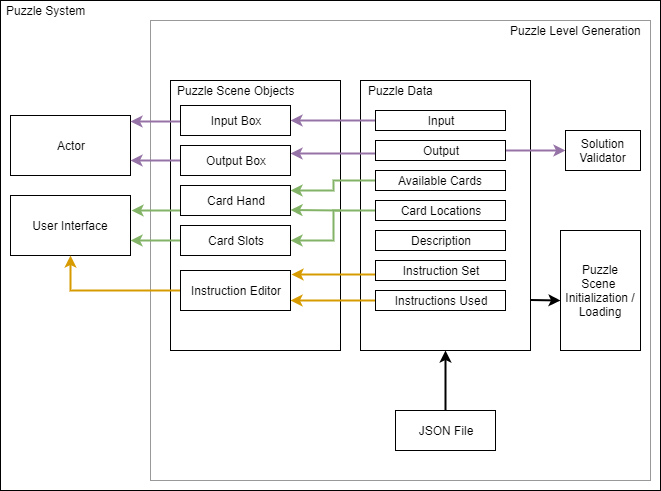
\includegraphics[scale=0.6]{Diagrams/puzzle_system_diagram.png}
\end{figure}
\vfill
\clearpage

The responsibilities of the puzzle system are as follows:

\begin{itemize}
	\item Presenting input to the player.
	\item Determining the expected output the player is responsible for generating
	\item Deciding the question we can ask the player
	\item Offering allowed operations the player can perfrom to solve the puzzle
	\item Loading an initial puzzle scene specific to each puzzle level
	\item Saving a puzzle scene state for a specific level when the player leaves
	\item Loading saved puzzle scene states for each level a player had previously attempted
\end{itemize}

Here are the main components of the Puzzle Scene that rely on the Puzzle System:

\begin{itemize}
	\item Input / Output (I/O)
	\begin{itemize}
		\item Input Box
		\item Output Box
		\item I/O Data (numbers)
	\end{itemize}

	\item Game Cards
	\begin{itemize}
		\item Player Card Hand
		\item Card Slots
	\end{itemize}

	\item Instruction Area
	\begin{itemize}
		\item Instruction bank
	\end{itemize}
\end{itemize}

Note:\\

While the Game Cards and the Instruction Area fall under the User
Interface System, there are certain parts of these components that rely on
the Puzzle System’s level generation functionalities. Only that relationship
will be mentioned here. Refer to the User Interface System for a more detailed
look at these game components.

\subsubsection{Puzzle Level Generation}
When a level is chosen to be played by the player, the puzzle system controls
which game objects get loaded on to the puzzle scene. This process is handled
by a puzzle generation script that reads JSON data associated to the specific
level that was chosen.

\subsubsection{Level Initialization/Loading}
The generator will either load or initialize a puzzle level depending on whether
or not the player has previously attempted to solve the puzzle level. This
decision process is exemplified in Figure \ref{fig:json_decision_diagram}.\\

If the JSON file does not exist, the player has not ever attempted the chosen level before. The
generator will then need to call upon a level initialization script that will
create a JSON file for the level that represents it's initial state. After the file
is written, it's data is loaded by the generator and the puzzle scene is loaded.
This sequence is shown in Figure \ref{fig:level_initialization_diagram}.\\

If it JSON file does exist, the generator simply skips the initialize step and
loads the puzzle scene state based on the file that was found for the level (as
shown in Figure \ref{fig:level_loading_diagram}).\\

This flow of control combines initialization and loading processes in order to simplify
the entire scheme. The only difference between the two is the possible need to
initially create a level's JSON file, but that created file, or the one that already
existed under the same name, is always loaded by the generator.\\

When a game is ran for the first time, there will be no JSON files associated to
ANY level. This means that the level initialization script will be invoked each time
the player opens a new level, as expected.\\

\begin{figure}[!hb]
  \caption{Puzzle Level Initialization/Loading Decision}
  \label{fig:json_decision_diagram}
  \centering
  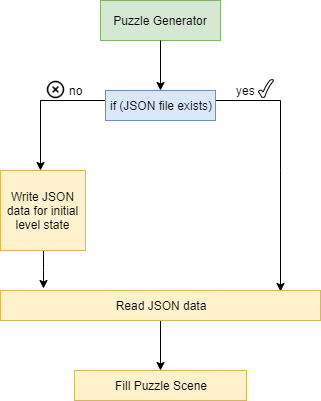
\includegraphics[scale=0.9]{Diagrams/json_decision_diagram.png}
\end{figure}
\vfill
\clearpage

\begin{figure}[!hb]
  \caption{Puzzle Level Initialization}
  \label{fig:level_initialization_diagram}
  \centering
  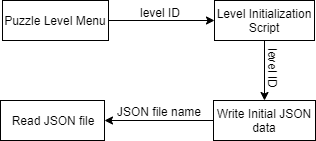
\includegraphics[scale=0.9]{Diagrams/level_initialization_diagram.png}
\end{figure}

\begin{figure}[!hb]
  \caption{Puzzle Level Loading}
  \label{fig:level_loading_diagram}
  \centering
  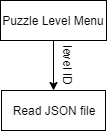
\includegraphics[scale=0.9]{Diagrams/level_loading_diagram.png}
\end{figure}
\vfill
\clearpage

\subsubsection{Level Saving}
When the player decides to leave a puzzle level (exiting the game, returning to the
level menu, etc), the puzzle system saves the state of the current level by writing
to the JSON file associated to it. Figure \ref{fig:level_saving_diagram} shows this process.

\begin{figure}[!hb]
  \caption{Puzzle Level Saving}
  \label{fig:level_saving_diagram}
  \centering
  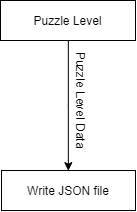
\includegraphics[scale=0.9]{Diagrams/level_saving_diagram.png}
\end{figure}

\subsubsection{JSON File Format}
The JSON file is serialized using a PuzzleData object that contains information
needed to fill the puzzle scene. This data can separated into two categories:\\

Data Needed for Level State Initialization:
\begin{itemize}
  \item Initial cards in hand
  \item Number of register cards available
  \item Number of stack cards available
  \item Number of queue cards available
  \item Number of heap cards available
  \item Input size
  \item Instruction set
  \item Puzzle description
\end{itemize}

Data Needed for Loading a Previous Level State:
\begin{itemize}
  \item Card placement
  \item Cards in hand
  \item Instructions in editor
\end{itemize}

\subsubsection{Input}
The puzzle system is in charge of filling the puzzle scene's input box with data
that is necessary for the chosen level. As shown by Figure \ref{fig:Puzzle_System_Input_Overview}, the puzzle generator
takes an input size, n, from the JSON file, and randomly generates an array of n
numbers that is used to fill the input box with corresponding data. A more visualized
look at how the input box game object is filled is shown in Figure \ref{fig:Puzzle_System_Input_Same_Before}.\\

\begin{figure}[!hb]
  \caption{Puzzle System: Input Overview}
  \label{fig:Puzzle_System_Input_Overview}
  \centering
  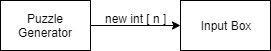
\includegraphics[scale=0.9]{Diagrams/Puzzle_System_Input_Overview.png}
\end{figure}

The puzzle system is responsible for giving the actor the correct data from the
input box when it is needed. The actor can make an input request to the input box.
The system will simply return the top-most element from the input box to the actor entity, along with the
numerical data that is associated with it behind the scenes (see Figure \ref{fig:Puzzle_System_Input_Actor}).\\

Note:\\

If the actor make an input request to an empty input box, the puzzle system
will return NULL.\\

The input box has a fixed number of input items that can fit inside (5 in our examples).
Sometimes the size of the input stream can be larger than the size of the input box
itself. In this case, the input box works as a queue. If we had an input stream of
size 6, the 6th element would be hidden until the top-most element of the input box
is removed by the actor. All of the elements below will move up a slot and the
hidden 6th element would then appear at the bottom, as shown in Figure \ref{fig:Puzzle_System_Input_Overload_Before} and
Figure \ref{fig:Puzzle_System_Input_Overload_After}.\\

If the input stream is the same size as the input box, or if the actor has removed
enough numbers from a larger stream and there are no more slots to fill, the input numbers
behave only slightly differently. Figure \ref{fig:Puzzle_System_Input_Same_Before}
and Figure \ref{fig:Puzzle_System_Input_Same_After} show how the numbers below will move up a slot, like before,
but the bottom slot will be left empty.\\

\begin{figure}[!hb]
  \caption{Puzzle System: Input-Box/Actor Communication}
  \label{fig:Puzzle_System_Input_Actor}
  \centering
  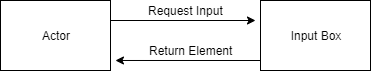
\includegraphics[scale=0.9]{Diagrams/Puzzle_System_Input_Actor.png}
\end{figure}

\begin{figure}[!hb]
  \caption{Puzzle System: Input-Box Overloading (before)}
  \label{fig:Puzzle_System_Input_Overload_Before}
  \centering
  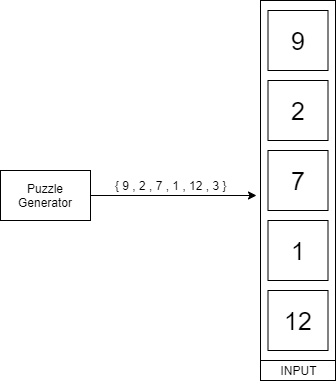
\includegraphics[scale=0.9]{Diagrams/Puzzle_System_Input_Overload_Before.png}
\end{figure}

\begin{figure}[!hb]
  \caption{Puzzle System: Input-Box Overloading (after)}
  \label{fig:Puzzle_System_Input_Overload_After}
  \centering
  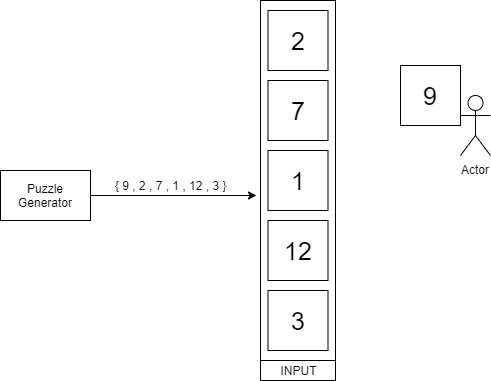
\includegraphics[scale=0.9]{Diagrams/Puzzle_System_Input_Overload_After.png}
\end{figure}
\vfill
\clearpage

\begin{figure}[!hb]
  \caption{Puzzle System: Input-Box Same Size (before)}
  \label{fig:Puzzle_System_Input_Same_Before}
  \centering
  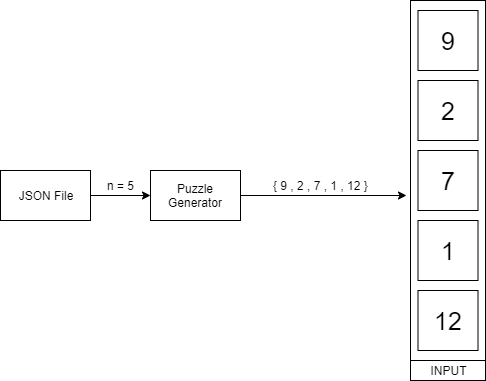
\includegraphics[scale=0.9]{Diagrams/Puzzle_System_Input_Same_Before.png}
\end{figure}

\begin{figure}[!hb]
  \caption{Puzzle System: Input-Box Same Size (after)}
  \label{fig:Puzzle_System_Input_Same_After}
  \centering
  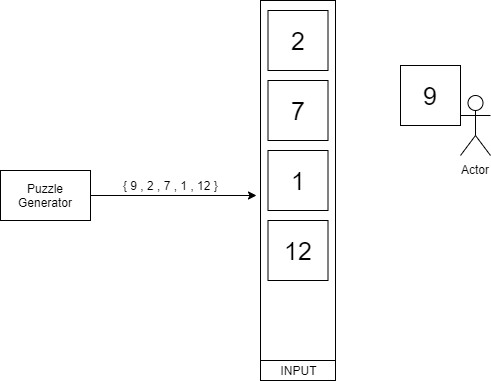
\includegraphics[scale=0.9]{Diagrams/Puzzle_System_Input_Same_After.png}
\end{figure}
\vfill
\clearpage

\subsubsection{Output}
